\documentclass[thesis.tex]{subfiles}
\begin{document}
\chapter[Introduction]{Introduction}
\label{chap:intro}

Pancreas cancer is a disease of great importance.  Despite being relatively uncommon, the exceptional lethality of most pancreas cancers makes them the 5th most frequent cause of cancer death in Australia~\cite{CAN88}.  The most common and aggressive form of pancreas cancer is \gls{PDAC}, which currently carries a five year survival rate of approximately $5\%$~\cite{CAN65}.  This dire prognosis has remained largely unchanged over the past thirty years~\cite{CAN65, SEER2014}, highlighting how little success the tools of modern molecular oncology have had in treating this poorly-understood disease.  \gls{PDAC} is a challenging disease to study, and relatively little is known about its molecular basis.  This may soon change: current cancer genome projects have now accrued large cohorts of \gls{PDAC} samples and clinical data, finally enabling the systematic dissection of this serious malignancy.  The work described here used these new data to gain a better understanding of why \gls{PDAC} is so aggressive, and in particular why some patients survive a relatively long time, whereas others succumb quickly to their disease.  Knowledge of the biological processes that mirror patient survival can improve patient staging and disease management in the medium term, and highlights target areas for the development of more effective therapies against this difficult disease.

Pancreas cancer is the most aggressive common malignancy, with a worse survival rate than even mesothelioma~\cite{CAN65}.  The exceptionally poor prognosis of pancreas cancer means that although it is the 12th most commonly-diagnosed cancer in Australia, it is the 5th most common cause of cancer death; worldwide, almost \fcardinal{360000} deaths are expected to occur to pancreas cancer in 2015~\cite{GLOBOCAN2015}.
%Although some genetic syndromes predispose to PDAC~\cite{TODO}, the majority of cases are thought to be sporadic, with smoking, heavy alcohol consumption, and obesity known environmental risk factors~\cite{TODO}.
The majority of pancreas cancers are \gls{PDAC}, a malignancy believed to originate in the exocrine compartment of the pancreas~\cite{TODO}.  \gls{PDAC} is strikingly resistant to treatment, and modern molecular oncology has yet to make much of an impact on the disease: despite extensive research, survival with pancreas cancer has not greatly improved in the last thirty years (\fref{fig:intro-historical-all-surv}).

\begin{figure}[!htbp]
\centering
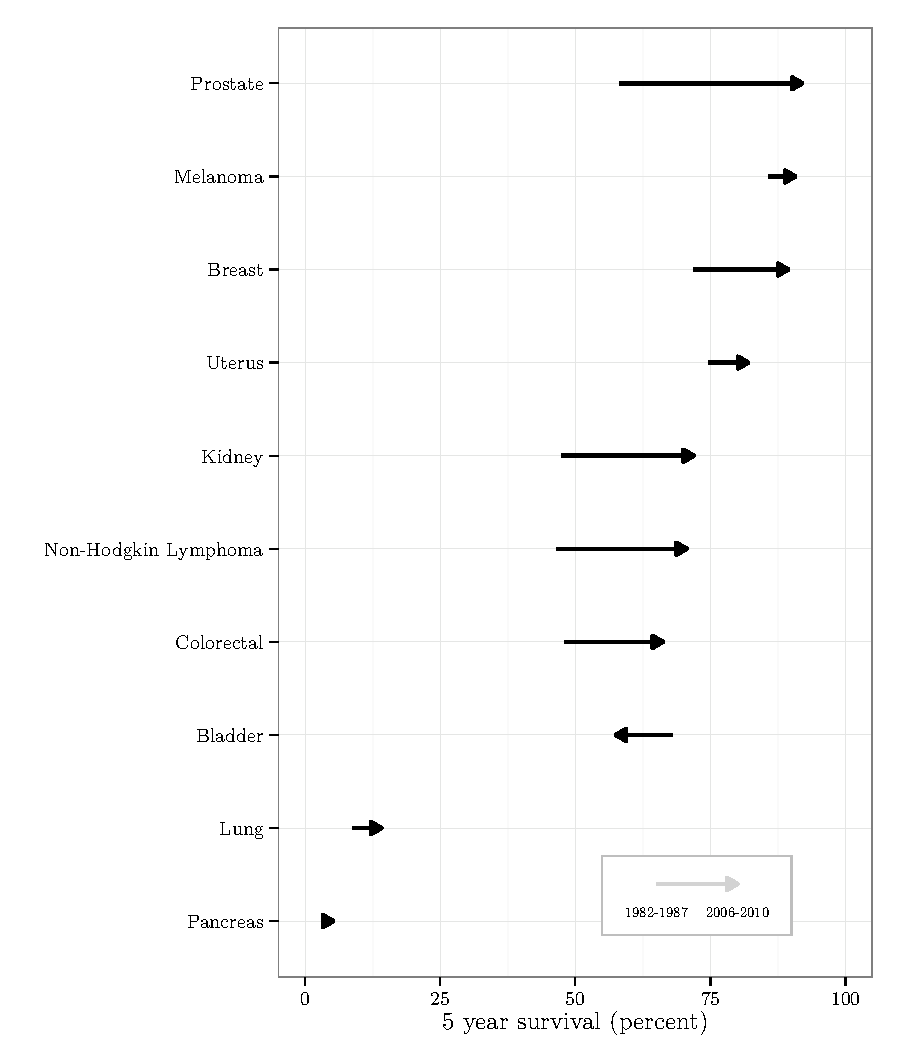
\includegraphics[width=.9\linewidth]{analysis/intro/figure/historical-survival-all-1}
\caption[Historical survival rates of common cancers]{Changes in survival rates for common cancers in Australia between 1982-1987, and 2006-2010.  The cancers shown are the ten most common by incidence; arrows move from the 1982-1987 survival rates to the 2006-2010 rates.  Most cancers had substantial increases in patient survival between the 1980s and the 2000s; pancreas cancer was an exception, with survival rates barely changing over the past 30 years.  Source: AIHW cancer survival and prevalence \cite{CAN65}}\label{fig:intro-historical-all-surv}
\end{figure}

The current standard of care for \gls{PDAC} is based on resection of the primary tumour, with accompanying chemotherapy or chemoradiotherapy~\cite{Editors2015}.  Unfortunately, resection is seldom possible, as approximately $80\%$ of patients present either with metastatic disease, or tumours that are too locally involved to safely resect~\cite{TODO}.  Even in the best case of a complete resection of a localised tumour, followed by thorough adjuvant chemotherapy, most patients will relapse with distant metastases that are ultimately fatal~\cite{Barugola2007}.  From this, two points are evident: even a complete resection rarely removes all disease, and current chemotherapy regimes are incapable of destroying the remaining transformed cells.  Little ground can be made on the first point, as the residual disease is likely due to the presence of undetected micro-metastases, which would be impossible to resect.  To address the second point, and improve the outcomes of patients with \gls{PDAC}, more effective chemotherapy regimes need to be developed.  This need is especially acute, as surgery to remove local \gls{PDAC} is a major procedure with significant associated morbidity~\cite{Ho2005}, and currently many patients who undergo resection receive little benefit from it.  To date, efforts to find improved chemotherapy for \gls{PDAC} have been hampered by a poor understanding of the molecular nature of \gls{PDAC}, and the challenges particular to the study of this disease.

\gls{PDAC} cancer is challenging to study.  It is a relatively rare cancer, in a tissue that is difficult to access, and unethical to biopsy in healthy people.  Additionally, very few samples of early \gls{PDAC} are available, as the disease is usually only diagnosed at an advanced stage, and therefore the early stages of \gls{PDAC} carcinogenesis have been particularly challenging to map~\cite{TODO}.  Molecular investigations are hampered by the presence of large quantities of desmoplastic stroma in bulk tumour samples; this stroma often significantly outnumbers the transformed epithelial cells, and dominates biomarker signals in the tissue~\cite{Collisson2011}.  Mouse models of \gls{PDAC} have been developed, that appear to recapitulate aspects of human disease \cite{TODO}.  However, a number of alternative models exist, with differing molecular characteristics ~\cite{TODO}, and it's unclear which, if any, is a suitable proxy for the human disease.

TODO: What \emph{did} we know about its molecular basis?  Generally not much.  Putative defined string of events, but limitation is that these were cross-sectional.  Debate over cell of origin.  The picture up until a few years ago was that PDAC is a relatively homogeneous disease, with few linked mutations.  BUT outcome variation is quite high -- how can this be if the disease is so homogeneous?  Interaction with env could be it, but perhaps there's more to the story.  Collisson subtypes BUT udissected, no genomic link, and minor survival difference -- how relevant are they in actual tumours?  They don't explain the surv variability that well anyway.  But the difficulties inherent in PDAC meant that we may have missed it.

New large-scale cancer genome efforts promise to finally establish the molecular nature of \gls{PDAC} in man.  Combined, \gls{TCGA} and the \gls{ICGC} have accrued approximately \fcardinal{1000} cases of \gls{PDAC}, with extensive linked molecular measurements and clinical annotation.  These projects are still in progress, but early analyses of data to date have indicated that \gls{PDAC} is a relatively genetically homogeneous disease~\cite{Biankin2012}, with the primary genetic variation between tumours being in the structural stability of their DNA~\cite{Waddell2015}.  This diversity in genomic stability is an exciting result, which immediately suggests a therapeutic direction~\cite{Waddell2015}, but is unlikely to be the last word in \gls{PDAC} subtypes.

Subtype information is often challenging to learn from genomic data, as these data can have low sensitivity, and a number of genetic alterations can result in the very similar changes in biological behaviour.  \Gls{GEX}, on the other hand, is relatively easy to quantify accurately, and serves as a composite signature of biological state that is particularly well suited to elucidating subtypes and molecular status~\cite{Ray2014}.  Examination of the \gls{ICGC} genomic alterations~\cite{Biankin2012, Waddell2015} suggests that \gls{PDAC} is either a very homogeneous disease, with only one subtype, or an extraordinarily heterogeneous one, with dozens.  However, this conclusion is plausibly due to the focus of those analyses on genetic alterations; to date the \gls{GEX} data generated by those studies has been neglected.  A careful analysis of the \gls{GEX} data available for \gls{PDAC}, in the spirit of early very successful work in breast cancer, promises to define disease subtypes of \gls{PDAC} of biological interest or clinical relevance.



And now enter me.  Why is this cancer so aggressive?  Why do some patients survive so much longer than others?  It looks from earlier work that the cancers are all basically the same, yet the difference in outcome contradicts this.  Perhaps the effect's not at the genome level.  The best way to dissect this is to get at GEX signatures -- could the GEX give us some insight on what is going on?

What can we do with this information?  First of all it gives better insight into the biology of survival.  This can be immediately used to identify biomarkers of outcome for better stratification and management.  Enter chapters 3 & 4.  But ultimately it leads to better understanding of the disease, not only academically, but also to indicate fresh directions for therapy.

\begin{figure}
\centering
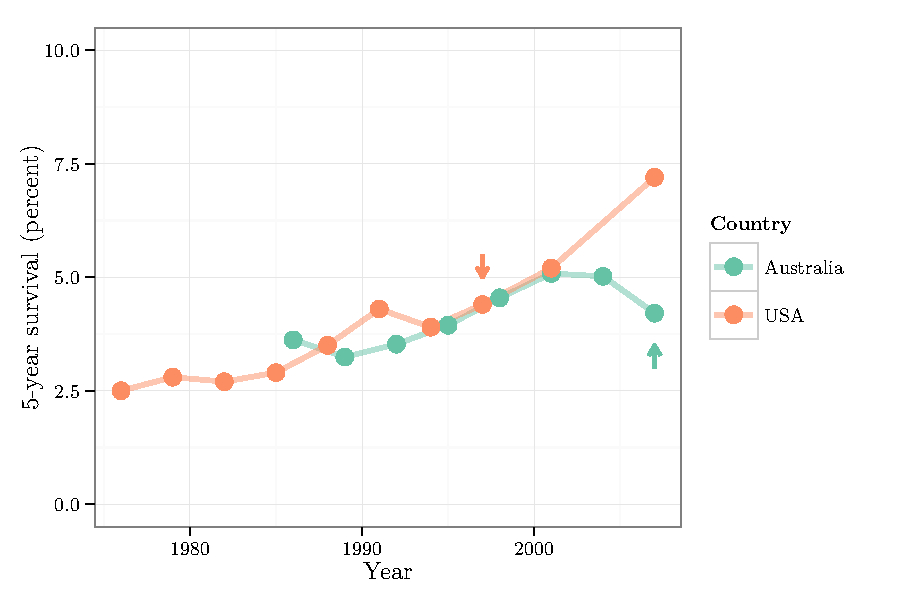
\includegraphics[width=.9\linewidth]{analysis/intro/figure/historical-survival-pdac-2}
\caption[Historical survival rates of pancreas cancer]{Pancreas cancer 5-year survival rates have remained largely stable over time.  Arrows indicate the year of regulatory approval for the use of gemcitabine adjuvant chemotherapy in each country.  Sources: AIHW cancer survival and prevalence \cite{CAN65}, and NCI SEER CSR \cite{SEER2014}}\label{fig:intro-historical-panc-surv}
\end{figure}

\cite{CAN65}

\end{document}
